\chapter{多変数関数の微積分}
さっきまでやってきたのは,1変数関数に関する微分積分学である.
しかし,物理量は1つの変数で決められるようなものはあまりない.変数が足りないのである.
複数の数に対して1つの数を対応させるような対応関係のことを\emph{多変数関数}
\index[widx]{たへんすうかんすう@多変数関数}というのだが,
この多変数関数に関しても微分積分学を考えたい.しかし,たくさんある変数のうちどれを追いかけたらいいのかよくわからない.
というわけで,まずは1つの変数にのみ着目し,あとの変数は定数だとみなしてしまうことにしよう.
このときに使うのが偏微分である.
偏微分を学ぶ前に,とりあえず多変数関数について確認しておこうか.
\section{多変数関数}
おそらく,読者の方々が高校生の間に扱ってきたのは独立変数を1つだけ持つ1変数関数である.
高校までの物理で扱ったのもおそらく1変数関数だけである.
時間$t$での物体の位置$x(t)$だとか,位置$x$での物体のポテンシャルエネルギー$V(x)$などがあっただろう.
しかし,物理量を扱ううえで,これではまずいのである.
例えば熱力学では,ある系の圧力$p$は,その系の体積$V$と温度$T$を決めてしまえばただ1通りに定まる.
だが,体積だけ,あるいは温度だけを決めても圧力は決まらない.
関数と似ているだろう.この場合,圧力は温度と体積の関数ということになる.
圧力$p$は$p(V, \, T)$と表せるのである.
この例では独立変数が2つある.温度と体積はそれぞれ勝手に動く.
一方,例えば温度を決めたとしても,それによって体積に何らかの制限がかかることはない.
``独立''変数というのはそういう意味である.
電磁気学での例も出しておこう.例えば,空間の電荷密度$\rho$は,位置と時間を決めれば値が決まる.
こういうと変数が位置と時間の2つのように聞こえるが,実際は4つの独立変数を持つ.
それは,位置が3つの変数によって決まるからだ.$x$座標,$y$座標,$z$座標を決めねば位置は決まらない.
だが,位置を決めれば電荷密度が決まるといえるかといえばそうではない.
ある場所の,基準の時間から1秒経ったときの電荷密度と3秒経ったときの同じ場所での電荷密度は同じとは限らない.
空間の電荷が移動していれば,電荷密度は時間とともに変化するからだ.
電荷密度は$x, \, y, \, z$そして時間$t$の4変数関数であるというわけだ.

さて,多変数関数の概念が何となく理解できたところできちんと定義しておこう.
$n$個の数$ x_1, \, x_2, \, \cdots , \, x_n $の値が確定したとき,もう1つの数$y$の値が
ただ1つに確定するような対応規則が与えられたとき,
そのような対応規則のことを\textbf{$n$変数関数}と呼ぶ.
\emph{多変数関数}\index[widx]{たへんすうかんすう@多変数関数|textbf}というのは,
値を決めるのに2つ以上の独立変数の値を要求する関数のことである.
そして,最初に決める変数(ここでは$ x_1, \, x_2, \, \cdots , \, x_n $のこと)を\emph{独立変数}
\index[widx]{どくりつへんすう@独立変数},
独立変数に対応して決定される変数(ここでは$y$のこと)を\emph{従属変数}
\index[widx]{じゅうぞくへんすう@従属変数}という.
$n$変数関数のことをよく$f$という記号で表すことが多い.
そして,独立変数の値を$ x_1, \, x_2, \, \cdots , \, x_n $に決定したとき,これらの数に対応する従属変数の値を
\begin{align*}
f( x_1, \, x_2, \, \cdots , \, x_n)
\end{align*}
と表す.
もし$x_1, \, x_2, \, \cdots , \, x_n$に対応する従属変数が$y$と表されていれば,それは
\begin{align}
y = f(x_1, \, x_2, \, \cdots , \, x_n)
\label{eq:nhensu}
\end{align}
というように表されるのである.
特に,2変数関数のときには独立変数を$x, \, y$と書き,従属変数を$z$と書いて
\begin{align}
z = f(x, \, y)
\label{2hensu}
\end{align}
と表すことが多く,3変数関数の場合には独立変数を$x, \, y, \, z$と書き,従属変数を$u$と書いて
\begin{align}
u = f(x, \, y, \, z)
\label{eq:3hensu}
\end{align}
と書き表すことが多い.また,対応関係を表す記号(ここでは$f$としている)は使わずに,
直接$z(x, \, y)$や$u(x, \, y, \, z)$と表してしまうことも多い.
ここで注意しなければならないのは,
独立変数や従属変数を表すのに使っていた記号はあくまでシンボルであるということである.
関数というのは数(2変数以上の場合には数の組)と数との対応規則であって,
$y$だの$x$だのといった文字で表された具体的な式のことではないのである.
\footnote{実は,このような解釈に至ったのはけっこう最近のことだったりする.}
とはいえ,やっぱり厳密に区別するのもめんどくさいので
``2変数関数$f(x, \, y)$''だとか``関数$u(x, \, y,\, z)$''などというようにといってしまうことも多い.
普通の本だとこういう表記はたくさんあるはずだ.本書にもたくさんある.

\begin{itembox}[l]{検討}
さっきまで書いていた関数の定義は,中学校や高校の教科書に書いてあるような定義とは少し違うはずである.
君たちの家にある中学校や高校の数学の教科書に書いてある関数の定義を調べ,
本書に記した定義と何がどう違うかをまとめよ.
\end{itembox}
物理をやるうえでは関数が数(の組)と数との対応規則であることを知らなくともどうにかなることが多いのだが,
やはり自分がよく使っているものの正確な定義くらいは知っておきたいものである.
\footnote{ここで,対応規則という言葉がひどく曖昧に思えたら一人前といっていいだろう.}
\newpage
\subsubsection{2変数関数のグラフは曲面を表す}
1変数関数$f(x)$において,実数$x$とそれに対応する値$f(x)$のペア$(x, \, f(x))$全体の集合は,
このペアを点の座標と考えることにより,曲線とみなせるのであった.
$x$軸上の各点$(x, \, 0)$に対して$f(x)$という高さを対応させ,
それを平面上に図示したのが図\ref{fig:f(x)}である.
\begin{figure}[h]
 \centering
 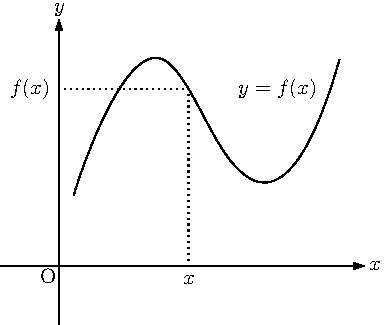
\includegraphics[width=5.8cm]{picture/henbibun1.pdf}
 \caption{1変数関数$y=f(x)$のグラフ}
 \label{fig:f(x)}
\end{figure} 

もちろん,$(x, \, f(x))$というペア全体の集合が曲線とみなせるのは,
$f$がなにかしらの良い性質を持っているときだけなのであるが,
物理で扱う関数はほとんどが滑らかさというとても良い性質を持っていることが多い.
あんまり細かいことは気にする必要はないということだ.

次に,2変数関数$f(x, \, y)$について考えよう.2つの実数$x, \, y$とそれに対応する値$f(x, \, y)$のペア
$(x, \, y, \, f(x, \, y))$を座標と解釈すれば,このペア全体の集合は曲面を表すことになる.
$xy$平面上の各点$(x, \, y, \, 0)$に対し,$f(x, \, y)$という高さを対応させていると考えるのである.
このことを空間上に図示したのが図\ref{fig:f(x,y)}ということになる.
\newpage
\begin{figure}[h]
 \centering
 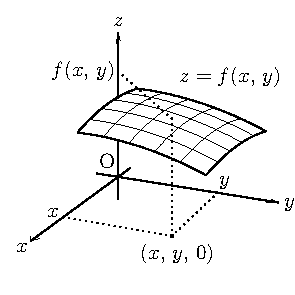
\includegraphics[width=5.8cm]{picture/henbibun2.pdf}
 \caption{2変数関数$z=f(x, \, y)$のグラフ}
 \label{fig:f(x,y)}
\end{figure} 
この場合も曲面とはとても思えないような変な関数を用意することもできるのだが,
話がややこしくなるのでそういうことはやめておくことにする.

この調子で3変数以上の関数についても考えることができそうだが,
3変数関数のグラフは4次元空間に存在するものであり,
これを人間の目に見える形で図示するのは不可能である.
\footnote{世の中には4次元空間が``見える''人が存在するようである.}
\subsection{陰関数}
関数というのは2つの量の関係を表すのであったが,どんな関係でも表せるというわけでもなく,
独立変数の値が決定されれば従属変数の値がただ1つに決定されるというような関係しか表せないのであった.
\footnote{しかし,従属変数の値が決定されても独立変数の値がただ1つに決定される必要はない.}
1変数関数のグラフは平面曲線を表し,2変数関数のグラフは空間曲面を表すのだが,
逆に,平面上の曲線すべてを1変数関数で表すことはできないし,
空間の曲面すべてを2変数関数で表すことはできない.
円や球面といった図形を考えてみればわかるはずだ.

このような曲線,曲面は単に$x, \, y$もしくは$x, \, y, \, z$の方程式として表される.
円であれば方程式$x^2+y^2=r^2$,球面であれば方程式$x^2+y^2+z^2=r^2$というようになるのである.
場合によっては1つの図形を表すのに方程式が複数必要になることがある.
例えば空間に存在する直線を表す場合である.詳細は高校レベルであるから省かせてもらう.

結局のところ,平面上の曲線や空間上の曲面は,$f(x, \, y)=0$
や$f(x, \, y, \, z)=0$といった方程式の形で表せるのである.
この$f$は今度こそ関数である.よく見ると,曲線を表す場合には$f(x, \, y)=0$となり,
この方程式は曲面を表していた
2変数関数$z=f(x, \, y)$に対して$z=0$という条件を付け加えたものと解釈できる.
曲面の場合も同様である.

さて,方程式が与えられればそれを解くことができるであろう.
話を簡単にするためにも平面上の曲線が方程式$f(x, \, y)=0$で表されている場合について考えよう.
いま,方程式$f(x, \, y)=0$が与えられたとき,それを$y$について解けば$y=g(x)$という形になることが予想される.
しかしこの$g$は関数であるとは限らない.方程式の解は複数存在し得るからだ.
だが,この方程式の解をたった1つの関数で表そうとしたのがいけないのであって,
複数の関数を用いて表してみてはどうだろう.
複数の関数を用意すれば方程式$f(x, \, y)=0$の定める$x$と$y$の関係を
完全に再現することができるはずである.
それに加え,もし大域的に見て解が複数あったとしても,$x$や$y$の値を制限して局所的に考えれば,
$y$を$x$の関数としてただ1通りに表すことができることが知られている.
局所的には方程式$f(x, \, y)=0$の解は1つしかないということである.
\footnote{この事実は数学的にも重要であって,陰関数定理と呼ばれている.}
すなわち方程式{$f(x, \, y)=0$}で表されるような曲線は,
複数の関数をひとまとめにしたものであるとみなせるのである.

きちんと定式化しておこう.2つの変数$x, \, y$について,方程式$f(x, \, y)=0$
が与えられたとする.この方程式が定める曲線上の点$(a, b)$の十分近くにおいて,
この曲線がある1変数関数$g$を用いて$y=g(x)$のグラフであるとみなせるとき,
すなわち,$a$に十分近い任意の$x$に対して$f(x, \, y)=0$をみたす$y$がただ1つに定まるとき,
この対応関係$g$は点$(a, \, b)$近傍において定義される関数である.
このとき,$g$は方程式$f(x, \, y)=0$によって
\emph{陰伏的に定められる}といい,
$g$を方程式$f(x, \, y)=0$によって定められる
\emph{陰関数}\index[widx]{いんかんすう@陰関数}と呼ぶ.
また,方程式$f(x, \, y)=0$が定める陰関数が複数あるとき,
それぞれの陰関数のことをこの陰伏関数の\emph{分枝}\index[widx]{ぶんし@分枝}と呼ぶ.
曲線を複数の枝の集まりだとみなしたときに,それぞれの枝が陰関数だと思ってのネーミングである.

これに対し,通常の$y=f(x)$の形の関数のことを\emph{陽関数}\index[widx]{ようかんすう@陽関数}と呼ぶことがある.
この対応関係は明らかに(陽に)関数ですよという意味合いを強調したいのだろう.

\subsection{パラメータ表示}
さて,陰関数の次はパラメータ表示の話である.
``パラメータ''という言葉は聞いたことくらいはあるだろう.
パラメータという言葉は学問分野や文脈,\index[widx]{ぱらめーた@パラメータ}
果ては個人個人によって異なる意味合いで使われることがあり,
正確に定義しろと言われてもちょっと難しいものがある.
とはいえ,みんな好き勝手に使っているのかというとそうでもなく,
たいていは「考えている対象の何らかの特性を表す補助的な変数」くらいの意味で使っていることが多い.
これから話すのは``曲線・曲面のパラメータ表示''という文脈で一般に使われているパラメータの話である.

\subsubsection{曲線のパラメータ表示}
さてと,まずは曲線について考えよう.平面上にある曲線$C$を考える.
話を簡単にするためにも,$C$はある点Aから別の点Bを連続的に繋いだ曲線だとしよう.
ある点Pを,点Aから出発して曲線$C$に沿って点Bまで動く点であるとしよう.
どのくらい動いたかは何らかの変数$t$によって定められているとしておく.
$t$が$a$から$b$まで動くとすれば,$t=a$ではPはAと一致し,$t=b$ならPはBと一致し,
$t$が増加するにしたがってPが曲線$C$上をAからBに向かって動いていくようなイメージである.
このとき,$t$が決まれば点Pがどこにあるかが確定する.
すなわち,点Pの座標は$t$の関数(っぽいもの)であるといえるのである.
平面上の点の座標というのは$x$座標と$y$座標で構成されるのだから,
点Pの座標が$t$で決まるというのは
Pの$x$座標と$y$座標がともに$t$の関数であるということと同値である.
その関数を$\varphi, \, \psi$としてみよう.
すなわち,点Pの座標を$(x, \, y)$としたときに,
\begin{align}
\left\{
\begin{aligned}
x & = \varphi(t) \\ 
y & = \psi (t) 
\end{aligned}
\right.
\qquad ( \, a \leq t \leq b \, )
\label{eq:parameta}
\end{align}
となるということである.
\footnote{本書では,不等号として$\leq, \, \geq$を採用している.
これらはそれぞれ$\leqq, \, \geqq$と同じ意味である.}
これを見ると,曲線$C$の各点$(x, \, y)$に対し,$a \leq t \leq b$なる実数$t$が
完全に1対1対応している.
\footnote{本当は$C$の端点などで1対1対応が崩れていても構わない.
この場合の点Aと点Bが一致する\emph{閉曲線}\index[widx]{へいきょくせん@閉曲線}の場合
などでこういうことが起こりうる.}
すなわち,式(\ref{eq:parameta})は曲線$C$を完全に表しているものといえる.
この実数$t$は曲線の形に何の影響も与えない.
重要なのは関数$\varphi, \, \psi$の形の方である.
すなわち,この$t$は曲線$C$を表すためのいわば補助的な変数といえるわけだ.
この$t$が冒頭に書いたパラメータの意味合いに合致していることがわかるだろう.
そういうわけで,式(\ref{eq:parameta})のことを$C$の
\emph{パラメータ表示}\index[widx]{ぱらめーた@パラメータ!ひょうじ@---表示}だとか
$C$の\emph{パラメトリック方程式}\index[widx]{ぱらめとりっくほうていしき@パラメトリック方程式|see{パラメータ}}
などと呼ぶ.
いまこの意味で使っているパラメータ(parameter)は
日本語では\emph{媒介変数}\index[widx]{ばいかい@媒介変数|see{パラメータ}}と訳される.
そういうわけで,高校の教科書なんかでは式(\ref{eq:parameta})のことを
$C$の\emph{媒介変数表示}
\index[widx]{ばいかいへんすう@媒介変数!ひょうじ@---表示|see{パラメータ}}と呼ぶのが普通である.

今回は曲線$C$が有限の範囲に収まっている状況を想定したが,
別にそうである必要もあるまい.パラメータの範囲を無制限にしてやれば,
はるか遠方にある$C$の点だって表現できるだろう.
今回そういう場合を考えなかったのは,はるか遠方まで曲線が伸びることを許すと,
どこを始点に据えたものかよくわからなくなるからである.
これは単に説明がしづらいということ以上の理由はない.
パラメータ表示ができるのは有限の範囲に収まった曲線だけだと勘違いしないように.

曲線のパラメータ表示はとても便利である.
まず,曲線上の点を考えるのに$t$という仮変数を用いることにより,
曲線を表す方程式が簡単に書けたりする.
これは,あとで実例を見せることにしよう.
次の点が最も重要であり,
さっきまではパラメータになにか特別な意味は持たせていなかったが,
あえてパラメータになんらかの意味を与えてやることにより,
具体的なイメージが容易になったり,そこに隠された性質が見えてきたりするのである.
これも実例を挙げて説明するのがいいだろう.次のパラメータ表示を見てほしい.
\begin{align*}
\left\{
\begin{aligned}
x & = v_0 \cos \theta \cdot t \\
y & = v_0 \sin \theta \cdot t - \frac{1}{2} g t^2 
\end{aligned}
\right.
\qquad ( \, 0 \leq t \, )
\end{align*}
ここで,$v_0, \, \theta , \, g$はただの定数であり,変化するのは$t$のみである.
もはやこの$t$が何を表していると解釈するかなどという野暮な問は不要だろう.
$t$を時間として解釈するのが自然である.
もちろんパラメータを消去して,
\begin{align*}
y = \tan \theta \cdot x - \frac{ g } { 2 v_0^2 \cos ^2 \theta} x^2
\end{align*}
と書くこともできるが,$t$を時間として解釈した以上,
この式は斜方投射を表していると理解しやすいのはパラメータ表示された式の方であろう.

\subsubsection{曲面のパラメータ表示}\index[widx]{ぱらめーた@パラメータ!ひょうじ@---表示}
次は,曲面のパラメータ表示についてである.
空間に存在する曲面$S$について考える.
曲線のときと同じように考えるとちょっと説明が面倒になるので,
今回は違った方法で考えてみよう.

$S$は空間に存在する曲面である.$S$の各点$(x, \, y, \, z)$に対し,
その点から$xy$平面に降ろした垂線の足全体の集合を$\pi$とおく.
\footnote{この集合$\pi$を$S$の$xy$平面への正射影という.}
\index[widx]{せいしゃえい@正射影}
$\pi$上の各点はすべて$xy$平面上の点だから,その座標$(x, \, y, \, 0)$
は2つのパラメータで表されるはずだ.
\footnote{$\pi$は曲線の無限個の和集合とみなせるから,
1つ目のパラメータでその点が$\pi$のどの曲線上にあるか指定し,
2つ目のパラメータでその点が曲線上のどこにあるかを指定するような
イメージをしてみれば納得できるだろう.}
そこでそのパラメータを$u, \, v$として,関数$\varphi, \, \psi$を用いて,
\begin{align*}
x = \varphi (u, \, v) \\
y= \psi (u, \, v)
\end{align*}
と表そう.なんでわざわざ平面上の点を$u, \, v$というパラメータを用いて表すのかといえば,
その方が後で楽だからである.
後の話を楽に進めるために,
$u, \, v$の組$(u, \, v)$と$\pi$上の各点$(x, \, y)$は完全に1対1対応している必要はないとしよう.
異なる2つの$u, \, v$の組$(u, \, v)$が$\pi$上の同じ点に対応させてもいいとするのである.

さて,$\pi$上の点が決まったとき,
その点と$x$座標と$y$座標が同じであるような$S$上の点を考える.
$\pi$上の各点に対し,その点と$x$座標と$y$座標が同じであるような$S$上の点は
ただ1つしかないといいたくなるが,いま,$S$は任意の曲面である.
そのため,$\pi$上の点を1つ決めても,その点と$x$座標と$y$座標が同じであるような
$S$上の点が複数ある場合があるのである.
この問題をパラメータが解決してくれる.
$\pi$上の各点に対し,その点と$x$座標と$y$座標が同じであるような$S$上の点
が複数あったとき,その数だけ異なるパラメータの組$(u, \, v)$に対して
同じ$\pi$上の点を対応させるとしよう.
そう考えれば,$S$上の点の$z$座標は$u, \, v$の関数として表すことができるのである.
そこでこの関数を$\xi$として,
\begin{align*}
z = \xi (u, \, v)
\end{align*}
と表すことにしよう. まとめると,$S$上の各点$(x, \, y, \, z)$は$u, \, v$という2つのパラメータを用いて
\begin{align}
\left\{
\begin{aligned}
x & = \varphi (u, \, v) \\
y & = \psi (u, \, v) \\
z & = \xi (u, \, v)
\end{aligned}
\right.
\label{eq:kyokuparameta}
\end{align}
と表せるのである.
これが曲面$S$のパラメータ表示である.
曲線から曲面になったときに,必要なパラメータが1つ増えたのである.

なお,空間に存在する曲線は,やはり1つのパラメータで
\begin{align}
\left\{
\begin{aligned}
x & = \varphi (t) \\
y & = \psi (t) \\
z & = \xi (t)
\end{aligned}
\right.
\end{align}
とパラメータ表示される.なぜかはもはや説明するほどでもないだろう.

長かったが,言いたいことは曲線はパラメータ1つで,
曲面はパラメータ2つでパラメータ表示できるということだけである.

\subsubsection{パラメータ表示された曲線の概形を描く}
さて,ここまで一般的な話しかしてこなかったので,
何か具体例が欲しいところである.
そこで,微分法の復習もかねて,パラメータ表示された曲線の概形を描いてみよう.

$a$を正の定数として,
$xy$平面上の曲線$C$が以下のようにパラメータ表示されているとする.
\begin{align}
\left\{
\begin{aligned}
x & = a ( 1 + \cos t) \cos t \\
y & = a ( 1 + \cos t ) \sin t
\end{aligned}
\right.
\qquad (0 \leq t \leq 2 \pi)
\label{eq: cardioid}
\end{align}
この曲線$C$を図示してみよう.
そのためにも,$t$の変化に対して$x, \, y$がどのように変化するかが知りたいところである.
すなわち,$t$に対する,$x, \, y$の変化率が知りたいのである.
それには,$x, \, y$を$t$で微分してやればいい.
\begin{align*}
\frac{ \mathrm{d} x} { \mathrm{d} t} 
& = a \cdot \Big( -\sin t \cos t + (1+ \cos t) (- \sin t) \Big) \\
& =  -a \sin t (1 + 2 \cos t) \, , \\
\frac { \mathrm{d} y} { \mathrm{d} t} 
& = a \Big( -\sin t \sin t + (1 + \cos t) \cos t \Big) \\
& = a ( 2 \cos ^2 t + \cos t -1) \\
& = a (\cos t +1) (2\cos t -1)
\end{align*}
今求めたのは$x, \, y$の$t$に対する変化率である.
従って,この値が正であれば$t$の増加に対して$x, \, y$は増加し,
負であれば$t$の増加に対して$x, \, y$は減少する.
もし0であれば$t$がほんの少し変化しても$x, \, y$の値は変化しないということになる.
これをもとに,$t$に対する$x, \, y$の変化を表にまとめよう.
このような表は$t$に対する$x, \, y$の\emph{増減表}\index[widx]{ぞうげんひょう@増減表}
と呼ばれるのであった.

\begin{table}[h]
\renewcommand{\arraystretch}{1.6}
\begin{flushleft}
\begin{tabular}{|c||c|c|c|c|c|c|c}
\hline
$t$ & 0 & $\cdots$  & $ \displaystyle \frac{ \pi }{3} $ & $\cdots$ 
& $ \displaystyle \frac{2}{3} \pi $ & $\cdots$ & \hspace{0.1cm} $\pi$ \hspace{0.1cm} \\ \hline
$ \displaystyle \frac{\mathrm{d} x }{\mathrm{d} t} $ & (0) & \multicolumn{3}{c|}{$-$} & 0 & $+$ & 0 \\ \hline
$x$ & $2a$ & $\leftarrow$ & $\displaystyle \frac{3}{4} a$ & $\leftarrow$ 
& $\displaystyle - \frac{1}{4} a$ & $\rightarrow$ & 0 \\ \hline
$\displaystyle \frac{\mathrm{d} y }{\mathrm{d} t}$  & (0) & $+$ & 0 &\multicolumn{3}{|c|}{$-$} & 0 \\ \hline
$y$ & 0 & $\uparrow$ & $ \displaystyle \frac{ 3 \sqrt{3} }{4} a$ & $\downarrow$ 
& $\displaystyle \frac{\sqrt{3} }{4} a$ & $\downarrow$ & 0 \\ \hline
\end{tabular}
\end{flushleft}
\end{table}
\vspace{-0.5cm}
\begin{table}[h]
\renewcommand{\arraystretch}{1.6}
\begin{flushright}
\begin{tabular}{c|c|c|c|c|c|}
\hline
$\cdots$ & $ \displaystyle \frac{4}{3} \pi$ & $ \cdots $ 
& $ \displaystyle \frac{5}{3} \pi $ & $ \cdots $ & $ 2 \pi $ \\ \hline
$-$ & 0 & \multicolumn{3}{c|}{$+$} & (0) \\ \hline
$\leftarrow$ & $ \displaystyle - \frac{1}{4} a$ & $\rightarrow$ 
& $ \displaystyle \frac{3}{4} a$ & $\rightarrow$ & $2a$ \\ \hline
\multicolumn{3}{c|}{$-$} & 0 & $+$ & $(+)$ \\ \hline
$\downarrow$ & $\displaystyle -\frac{ \sqrt{3}}{4} a $ & $\downarrow$ 
& $ \displaystyle -\frac{3\sqrt{3}}{4} a $ & $\uparrow$ & 0 \\ \hline
\end{tabular}
\end{flushright}
\end{table}
この表の意味はわかるだろう.$x$が増加・減少は$x$軸を歩くようなイメージで横向きの矢印で表しており,
$y$の増加・減少は$y$軸を歩くようなイメージで縦向きの矢印で表している.
この表から曲線$C$の概形がイメージできるだろうか? $t=0$に対応する点$(2a, \, 0)$からスタートして,
そこから$t$の増加に伴い増減表に書いたような進み方で進んでいく.
そうして最終的に$t= 2 \pi$に対応する点$(2a, \, 0)$に戻ってくるというわけである.
このことを頭に思い浮かべながら$C$の概形を描けば,
それは図\ref{fig:cardioid}のようになる.

\begin{figure}[h]
 \centering
 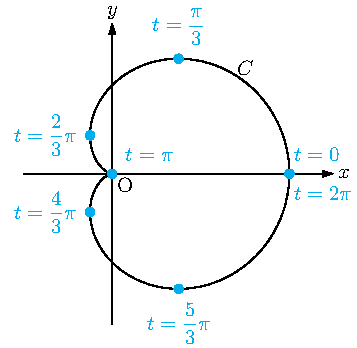
\includegraphics[width=5.5cm]{picture/henbibun3.pdf}
 \caption{曲線$C$の概形}
 \label{fig:cardioid}
\end{figure}

$x, \, y$の増減が変化する点とそのときの$t$の値を図に書き込んでおいた.
あまりたくさん情報を書き込みすぎると図が汚くなるので書き込む情報は最小限に抑えている.
ここまで書かれればさすがに理解できるだろう.

この曲線は\emph{カージオイド}\index[widx]{かーじおいど@カージオイド}と呼ばれる有名な曲線である.
名前くらいは聞いたことがあるかもしれない.
\begin{itembox}[l]{課題}
\begin{align*}
\left\{
\begin{aligned}
x & = a ( t - \sin t) \\
y & = a ( 1 - \cos t )
\end{aligned}
\right.
\qquad (0 \leq t \leq 2 \pi)
\end{align*}
とパラメータ表示された曲線の概形を描け.
ただし$a$は正の定数とする.
 \end{itembox}
なお,この曲線もこれまた有名な曲線で,\emph{サイクロイド}\index[widx]{さいくろいど@サイクロイド}
と呼ばれている.
物理を学んでいると,時々出くわすことがある曲線である.
名前くらいは覚えておいても損はないだろう.
\section{偏微分}
ここからやっと偏微分の話に入る.
多変数関数なら変数がいくつあってもここから先の話はまったく変わらないのだが,
ここは簡単のために3変数関数について考える.
$x, \, y, \, z$の3つの独立変数をもつ関数$f(x, \, y, \, z)$について考えよう.
この関数$f$というのは,$x, \, y, \, z$の3つの値を定めたときに
初めて$f(x, \, y, \, z)$という値が定まるような対応関係であった.
そこで,先に$y=b, \, z=c$と定めてしまおう.$x$の値がまだ定まっていないので,
$f$によって値が確定することはない.
しかし,ひとたび$x$の値を決めてしまえば$f$によって値が決定される.
これはまるで1変数関数のようである.
数$x$に対して$f(x, \, b, \, c)$を対応させるような関数を$g$とすれば,
\begin{align*}
g(x) = f(x, \, b, \, c)
\end{align*}
となる.$g$は1変数関数だから,これまでと同じように微分することができるはずだ.
もし関数$g(x)$が微分可能であれば,その導関数は
\begin{align*}
\frac{\mathrm{d}g}{\mathrm{d}x}
\end{align*}
と表せる.$g$は仮に用意した関数記号であったから,これを$f$に置き換えたいのだが,
$f$はもともと3変数関数であった.これを$g$という1変数関数に無理やり落とし込んでやったので,
普通の微分の記号を使うのはなんとなく気が引ける.
そこで,dを丸めたような記号$\partial$を用いて$g$の導関数を
\begin{align*}
\frac{\partial f}{\partial x} (x, \, b, \, c)
\end{align*}
と表してやろう.なにやら新しい記号が出てきたが,
その中身はいままでやっていた導関数とほとんど同じものである.
後ろに$(x, \, b, \, c)$と書いてあるが,
これは$y, \, z$をどの値に固定したかを忘れないために書いている.

さて,ここからが肝心なところである.さっき``$y, \, z$を固定した''と書いたが,
実際やったことといえばただ単に$y, \, z$を$b, \, c$と書き換えただけである.
言ってしまえば$b, \, c$という文字列を突っ込んだだけである.
我々は,常日頃から定数を表すときは$a, \, b, \,  c, \, \cdots$という記号列を使い,
変数を表すときは$x, \, y, \, z , \, \cdots$を使うという習慣をつけているためか,
ただ単に記号を替えただけで定数になったと思い込んでしまう.
しかしながら,真に重要なのはもはやそこではない.
我々が$b, \, c$などと書いてあるだけで定数と思い込んでしまうのであれば,
そもそも記号を書き換えずに$y, \, z$とそのまま置いておいて,
この$y, \, z$は定数だとかたくなに信じ込むようにすれば同じことである.
すなわち,$x$で微分するときだけ$y, \, z$を定数だと思い,
ひとたび微分が終わったら$y, \, z$をまた変数だと思うようにするのである.
わざわざ$\partial$という記号を採用したのはこのような意識を前面に押し出すためである.

さて,関数$f(x, \, y, \, z)$について,$y, \, z$を定数だと思って$x$について微分して得られる関数を
関数$f(x, \, y, \, z)$の$x$に関する\emph{偏導関数}\index[widx]{へんどうかんすう@偏導関数}といい,
\begin{align}
\frac{ \partial f}{\partial x}
\label{eq:xhenbibun}
\end{align}
と書き表す.
関数の偏導関数を求めることをその関数を(変数名を明示して)\emph{偏微分する}
\index[widx]{へんびぶんする@偏微分する}という.
さっきの例では関数$f(x, \, y, \, z)$を$x$で偏微分したのである.

1変数関数の微分の定義に沿って言えば,
関数$f(x, \, y, \, z)$を$x$で偏微分するというのは,次のような極限を求めることなのである.
\begin{align}
\lim_{\varDelta x \to 0} \frac{ f(x + \varDelta x , \, y, \, z) - f(x, \, y, \, z)}{\varDelta x }
\end{align}
$x$の変化$\varDelta x$のみを考え,$y, \, z$の変化を一切考慮していないのがミソである.

$f(x, \, y, \, z)$を
他の変数$y, \, z$で偏微分したときは
\begin{align*}
\frac{\partial f}{\partial y} \; , \; \frac{\partial f}{\partial z}
\end{align*}
というように書くのである.$y$で偏微分するときには$x, \, z$を定数とみなすことにして,
$z$で偏微分するときには$x, \, y$を定数かのように扱う.
また,どの変数を一定にしたかを強調するためにカッコをつけて右下におき,
\begin{align*}
\left( \frac{\partial f}{\partial y} \right)_{x, \, z}
\end{align*}
と書くこともある.この例では$x$と$z$を一定にしますよと書いてある.
これはどんな物理量を変数に据えるかを大事にする熱力学でよく見かける記法である.
電磁気学ではあまり使わないので本書でも使わない.

また,偏導関数を表すのに$f_x$や$f_y$などという記法を使うことがある.
\begin{align}
f_ x = \frac{\partial f}{\partial x} \, , \, f_ y = \frac{\partial f}{\partial y}
\label{eq:hendoukansusoeji}
\end{align}
こんな感じである.
これは便利なのでたまに使うことがあるだろう.

偏微分と1変数関数での普通の微分との違いを強調したいときに,今までやっていた1変数関数での微分を
\emph{常微分}\index[widx]{じょうびぶん@常微分}と呼ぶこともある.

また,$\partial$の読み方であるが,最近は``デル''と読むことが多い.他にも,dと同じ読み,つまり``ディー''と読んだり,
丸まったdというニュアンスで``ラウンド・ディー''と読んだり,
``パーシャル''と読むこともあるそうだ.
最近の傾向に合わせて``デル''と読んでおくのが無難である.
上の例でいえば``デル・エフ・デル・エックス''と読むのである.

さらに,常微分と同じように偏微分にも高階の偏導関数が考えられる.ただし,変数が多い分バリエーションが増える.
関数$f$を$x$で偏微分してから$y$で偏微分したとき,これを
$$
\frac{\partial^2 f}{\partial y \partial x}
$$
と書く.これは``デル・ツー・エフ・デル・エックス・デル・ワイ''と読めばよい.記号の由来が
$$
 \frac{\partial}{\partial y} \left( \frac{\partial f}{\partial x} \right)
 $$
 というところからきていると思えば書き方に納得できるだろう.
 $x$で偏微分してから$y$で偏微分する場合と,$y$で偏微分してから$x$で偏微分するのとでは結果が異なるかもしれない.
 しかし,物理で扱うような通常の関数では偏微分する順番は気にしなくてもよいことがわかっている.
 $$
 \frac{\partial^2 f}{\partial y \partial x} = \frac{\partial^2 f}{\partial x \partial y}
 $$
 が成り立つということである.
 同じ文字,たとえば$x$で2回偏微分したら,これは
 $$
 \frac{\partial^2 f}{\partial x^2}
 $$
 と書き表されることなる.読み方はいい加減いいだろう.常微分のときのdをデルと読み替えるだけである.
 
例によって,多変数関数の偏導関数に各点の座標を代入して得られる値は
\emph{偏微分係数}\index[widx]{へんびぶんけいすう@偏微分係数}と呼ばれる.
これも常微分のときとほとんど同じである.
\subsubsection{偏微分の具体例}
偏微分を具体的やってみよう.あまり複雑なものをやっても仕方ないので,ここでは3変数関数でやってみる.
独立変数を$x, \, y, \, z$として,$u=f(x, \, y, \, z)$の形の関数を考えることにする.
\label{ex:henbibun}
\begin{enumerate}
\item $u(x, \, y, \, z)=x^3+3x^2yz-2xyz^2+y^2-2z^3$とする. \\
$x$で偏微分するときには,$y, \, z$はただの定数とみなせばよい.
$$
\frac{\partial u}{\partial x} = 3x^2+6xyz-2yz^2 
$$
となる.$y$で偏微分するときには$x, \, y, \, z$は定数とみなすのだから
$$
\frac{\partial u}{\partial y} = 3x^2z-2xz^2+2y
$$
となるのである.$z$で偏微分するときも同様である.
$$
\frac{\partial u}{\partial z} = 3x^2y-4xy-6z^2
$$
というわけである.何をしているかわかるだろうか? よく考えてみてほしい.
2階微分も同様である.が,何で偏微分するかの組み合わせがある.
$x$で2回微分する場合は
$$
\frac{\partial^2 u}{\partial x^2} = 6x+6yz
$$
となるし,$x$で偏微分してから$y$で偏微分すれば
$$
\frac{\partial ^2 u}{\partial y \partial x} = 6xz-2z^2
$$
となり,順番を逆にすると,
$$
\frac{\partial ^2 u}{\partial x \partial y} = 6xz-2z^2
$$
となり,
$$
\frac{\partial ^2 u}{\partial y \partial x} = \frac{\partial ^2 u}{\partial x \partial y}
$$
が成り立っていることがわかる.偏微分する順番は普通の関数では気にしなくてよいということだ.
もちろん,何で何回微分したかが違えば結果は異なる.この例でも
$$
\frac{\partial ^2 u}{\partial y \partial x} \neq \frac{\partial^2 u}{\partial x^2}
$$
となっている.当然だが頭が混乱しだすとわからなくなるので冷静に読んでほしい.この例はこのくらいにして次にいってみよう.
\item $\displaystyle u(x, \, y, \, z) = \frac{1}{\sqrt{x^2+y^2+z^2}}$とする.\\
もうくどい解説はいいだろう.
\begin{eqnarray*}
\frac{\partial u}{\partial x} & = & \frac{\partial}{\partial x} (x^2+y^2+z^2)^{-\frac{1}{2}} \\
& = & -\frac{1}{2} (x^2+y^2+z^2)^{-\frac{3}{2}} \cdot 2x \\
& = & -\frac{x}{(x^2+y^2+z^2)^{\frac{3}{2}}}
\end{eqnarray*}
であるから,まったく同様にして,
$$
\frac{\partial u}{\partial y} = -\frac{y}{(x^2+y^2+z^2)^{\frac{3}{2}}} \; , \; 
\frac{\partial u}{\partial z} = -\frac{z}{(x^2+y^2+z^2)^{\frac{3}{2}}}
$$
であることがわかる.(各自計算せよ)
2階微分については課題にするので次の例に移るとしよう.
\item $u(x, \, y, \, z) = \exp (xyz)$とする.
$$
\frac{\partial u}{\partial x} = yz \exp (xyz)
$$
であり,これをさらに$x$で偏微分してみると
\begin{align*}
\frac{\partial^2 u}{\partial x^2} = y^2z^2 \exp (xyz)
\end{align*}
となる.
\label{ex:henbibun2}
\end{enumerate}

ここまでやれば偏微分の計算は平気だろう.やけにあっさり終わってしまったが,本当にこれくらいしか語ることがないのである.
さて,例でやり残した分は演習としよう.
\begin{itembox}[l]{問}
例にあげた3つの関数について,2階の偏導関数のうち,やり残したものをすべて求め,微分する順番が結果に影響しないことを確かめよ.
また,例2の関数について,
$$
\frac{\partial^2 u}{\partial x^2}+\frac{\partial^2 u}{\partial y^2}+\frac{\partial^2 u}{\partial z^2} = 0
$$
が成り立っていることを確かめよ.
\end{itembox}
\newpage
\subsection{偏微分係数の幾何学的解釈}
1変数関数のときには,微分係数というのはその点における接線の傾きを表しているのであった.
2変数関数の場合では,偏微分係数を考えるときに片方の変数を固定して
さも1変数関数であるかのように扱うのであった.
1変数関数であれば,そのグラフは曲線を表す.
さも曲面を座標軸に垂直な平面で切断し,その切り口を観察しているようなイメージである.
このように考えると,偏微分係数はその点における接線の傾きを表しているということになる.
しかし,同じ点であっても,固定する変数によって接線が2通り考えられる.
$x$に関する偏微分係数を考えるのであれば,その接線は$x$軸に平行で,
$y$に関する偏微分係数を考えるのであれば,その接線は$y$軸に平行であるということになる.

さて,空間に直線が2本あれば,それらの直線を含むような平面を考えることができる.
この平面は,関数$z=f(x, \, y)$のグラフにちょうど接するような平面である.
そういうわけで,この平面を曲面$z=f(x, \, y)$のその点における\emph{接平面}
\index[widx]{せつへいめん@接平面}と呼ぶ.
空間に存在する平面の方程式というのは$x, \, y, \, z$の1次式で表されるのであったから,
2変数関数における1次近似というのは曲面をその点における平面に近似するのだと解釈できる.
このことを念頭に置きながら次の全微分の解説を読んでほしい.
\newpage
\section{全微分}
偏微分というのは,多変数関数における独立変数のうち,どれか1つだけが変化する場合について考えるのだった.
しかし,そんな都合のいい状況はほとんどないだろう.すべての変数が動き回る状況を考えなくてはならない.
だが,それらは偏微分をうまく組み合わせることによって実現できてしまうのである.

とりあえず3変数関数$f(x, \, y, \, z)$について考えることにしよう.変数が増えてもやることは一緒である.
\subsubsection{``微分''ってなんだっけ?}
すべての変数を動かすといったのだが,まずはやっぱり1つの変数だけを動かそう.
$x, \, y, \, z$のうち$x$だけが微小量$\mathrm{d}x$だけ変化したとき,$f$の微小変化$\mathrm{d}f$は
$$
\mathrm{d}f = \frac{\partial f}{\partial x} \mathrm{d}x
$$
と表せるのだった.1変数関数のときに出てきた微分の式をちょっとアレンジしただけである.
わからない,あるいは覚えていないという人は,もう一度1変数関数の微分の解説を読んできてもらいたい.
いまは$x$だけを変化させた想定なので導関数の部分が偏導関数となっている.
ただし,微小変化の$\mathrm{d}f$や$\mathrm{d}x$は$\partial f$や$\partial x$などとは書かない.
$\partial$はあくまで偏微分を表すときにのみ使われる記号である.\footnote{領域$D$があったとき,
その境界という意味で$\partial D$という記号が使われることはある.ベクトル解析を本格的に勉強しようと思ったときにこのような記号法に出くわすかもしれない.}

同じように考えて,$y$だけが微小量$\mathrm{d}y$だけ変化したとき,$f$の微小変化$\mathrm{d}f$は
$$
\mathrm{d}f = \frac{\partial f}{\partial y} \mathrm{d}y
$$
と書き表せるし,$z$だけが微小量$\mathrm{d}z$だけ変化したとき,$f$の微小変化$\mathrm{d}f$は
$$
\mathrm{d}f = \frac{\partial f}{\partial z} \mathrm{d}z
$$
と書き表せるということである.式だけ見ていても何も見えてこない.どういう想定で立てられた式なのかをよく理解しておいてもらいたい.

\subsubsection{偏微分から全微分へ}
さて,$x, \, y, \, z$がそれぞれ$\mathrm{d}x, \, \mathrm{d}y, \, \mathrm{d}z$だけ微小変化したとき,
$f$の変化$\mathrm{d}f$はどのようになるだろうか? この$\mathrm{d}f$こそ
$f$の全微分と呼ばれるものである.

$x$,$y$,$z$は独立にそれぞれ勝手に動くのだった.ならば,先に$x$を動かし,さらに次に$y$を動かし,ついで$z$を
動かしても結果は変わらないのではないだろうか? それぞれの変化が微小なうちは,
その周辺での偏微分係数,つまり各変数に対する関数の変化率はすべてほとんど変化しないと考えられるからだ.
これをもとにして$f$の全微分を求めてみよう.まず,$x$を$\mathrm{d}x$だけ微小変化させた場合の
$f$の変化$\mathrm{d_1}f$は(これから他の変数も変化させるので区別する意味合いで添え字をつけている)
$$
\mathrm{d_1}f = \frac{\partial f}{\partial x} \mathrm{d}x
$$
となり,続いて$y$を微小量$\mathrm{d}y$だけ変化させた場合の$f$の
($x$が変化した分も合わせた)変化$\mathrm{d_2}f$は
$$
\mathrm{d_2}f = \mathrm{d_1}f + \frac{\partial f}{\partial y} \mathrm{d}y
= \frac{\partial f}{\partial x} \mathrm{d}x + \frac{\partial f}{\partial y} \mathrm{d}y
$$
となる.最後に$z$を微小量$\mathrm{d}z$だけ変化させれば,$f$の($x, \, y$が変化した分も合わせた)変化量$\mathrm{d_3}f$は
$$
\mathrm{d_3} f = \mathrm{d_2}f + \frac{\partial f}{\partial z}\mathrm{d}z = 
\frac{\partial f}{\partial x} \mathrm{d}x + \frac{\partial f}{\partial y} \mathrm{d}y 
+  \frac{\partial f}{\partial z}\mathrm{d}z
$$
となるわけである.まとめると,$x, \, y, \, z$が
それぞれ$\mathrm{d}x, \, \mathrm{d}y, \, \mathrm{d}z$だけ微小変化したとき,$f$の変化$\mathrm{d}f$は
\begin{eqnarray}
\mathrm{d}f =
\frac{\partial f}{\partial x} \mathrm{d}x + \frac{\partial f}{\partial y} \mathrm{d}y 
+  \frac{\partial f}{\partial z}\mathrm{d}z
\label{eq:zenbibun}
\end{eqnarray}
と書き表せるということである.ずいぶんときれいな式となった.これを$f$の
\index[widx]{ぜんびぶん@全微分}\emph{全微分}と呼ぶ.
それぞれの変数が単独で変化したとしたときの変化量を合計すればよいということである.
また,$x, \, y, \, z$が
それぞれ$\mathrm{d}x, \, \mathrm{d}y, \, \mathrm{d}z$だけ微小変化したとき,$f$の変化$\mathrm{d}f$が
式(\ref{eq:zenbibun})のように表せるとき,
$f$は\emph{全微分可能である}\index[widx]{ぜんびぶん@全微分!かのうである@---可能である}
という.全微分可能でない多変数関数ももちろんあるが,
物理で扱うことはあまりないだろうから気にしなくてもいいだろう.

ところで,数学書には全微分可能であることの定義がまったく違った形式で書かれているはずである.

\begin{itembox}[l]{定義}
関数$f(x, \, y, \, z)$が点$\mathrm{P}(a, \, b, \, c)$で全微分可能であるとは,定数$A, \, B, \, C$と
点$\mathrm{P}$の周りで定義され,かつ点$\mathrm{P}$で連続であり$\varepsilon(a, \, b, \, c)=0$
をみたすような関数$\varepsilon(x, \, y, \, z)$が存在して,関数$f(x, \, y, \, z)$が点$\mathrm{P}$の周りで
\begin{align*}
f(x, \, y, \, z) = f(a, \, b, \, c) + (x- a) \, A + (y-b) \, B + (z-c) \, C \\
+ d (\mathrm{P}, \, \mathrm{Q}) \,  \varepsilon(x, \, y, \, z)
\end{align*}
と書き表せることである.ここで,
点$\mathrm{Q}$の座標は$\mathrm{Q}(x, \, y, \, z)$であり,$d(\mathrm{P}, \, \mathrm{Q})$は
点$\mathrm{P}$と点$\mathrm{Q}$との距離である.つまり,
\begin{align*}
d( \mathrm{P} , \, \mathrm{Q} ) = \sqrt{ (x-a)^2+ (y-b)^2 + (z-c)^2 }
\end{align*}
である.
\end{itembox}
一見すると式(\ref{eq:zenbibun})とまったく違うように見えるが,実際はほとんど同じことを表している.
$x-a, \, y-b, \, z-c$はそれぞれ$x, \, y, \, z$の変化量である.
これが微小であれば,これらを$\mathrm{d}x, \, \mathrm{d}y, \, \mathrm{d}z$と書いてもいいだろう.
さらに,後ろの$d(\mathrm{P}, \, \mathrm{Q}) \, \varepsilon(x, \, y, \, z)$の部分は
点$\mathrm{P}$が点$\mathrm{Q}$が十分近ければとても小さな値となる.
$d(\mathrm{P}, \, \mathrm{Q}) \, \varepsilon(x, \, y, \, z)$
が連続関数だからである.
これは,$x, \, y, \, z$の変化が十分小さい,つまり微小であることとまったく同じことである.
すなわち,$x, \, y, \, z$の変化が微小であるとき,上の式は
\begin{eqnarray}
f(x, \, y, \, z) \approx f(a, \, b, \, c) + (x-a)A+(y-b)B+(z-c)C
\label{eq:zenbibunkinji}
\end{eqnarray}
と近似できることになる.
また,定数$A, \, B, \, C$はそれぞれ
\begin{eqnarray*}
A=\frac{\partial u}{\partial x} (a, \, b, \, c) \\
B=\frac{\partial u}{\partial y} (a, \, b, \, c) \\
C=\frac{\partial u}{\partial z} (a, \, b, \, c) 
\end{eqnarray*}
となる.後ろに$(a, \, b, \, c)$とついているのは
偏微分した後に$(x, \, y, \, z)=(a, \, b, \, c)$を代入してくれよということである.
こうなる理屈はわかるだろうか? まず式(\ref{eq:zenbibunkinji})の両辺を$x$で
偏微分した後に$(x, \, y, \, z)=(a, \, b, \, c)$を代入すれば$A$の式が得られ,
式(\ref{eq:zenbibunkinji})の両辺を$y$で
偏微分した後に$(x, \, y, \, z)=(a, \, b, \, c)$を代入すれば$B$の式が得られ,
式(\ref{eq:zenbibunkinji})の両辺を$z$で
偏微分した後に$(x, \, y, \, z)=(a, \, b, \, c)$を代入すれば$C$の式が得られるという具合である.
いまは$d(\mathrm{P}, \, \mathrm{Q}) \, \varepsilon(x, \, y, \, z)$の部分を無視して計算したが,
これを無視せず計算しようとすると少し面倒なことになる.しかし,結果は変わらない.
興味があればやってみてもいいだろう.
そして,$f(x, \, y, \, z)-f(a, \, b, \, c)$は$f$の変化量のことであり,
これが微小であるとして$\mathrm{d}f$と置き換えれば,式(\ref{eq:zenbibunkinji})
の成立はもはや近似的ではないとしてもよく,このとき式(\ref{eq:zenbibunkinji})は
$$
\mathrm{d}f =
\frac{\partial f}{\partial x} \mathrm{d}x + \frac{\partial f}{\partial y} \mathrm{d}y +  \frac{\partial f}{\partial z}\mathrm{d}z
$$
と書き換えられることになる.これは,式(\ref{eq:zenbibun})とまったく同じである.
全微分可能であることの2つの定義はほとんど同じことを述べていたということである.

ところで,私は1変数関数の微分のところで次のような定理を紹介したのだった.
\begin{itembox}[l]{定理}
関数$f(x)$が点$a$で微分可能であり,かつ$A = f'(a)$であるための必要十分条件は,
点$a$のまわりで$f(x)$が
$$
\lim_{x \to a} \varepsilon (x) = \varepsilon (a) = 0
$$
をみたすような点$a$のまわりで定義された関数$\varepsilon (x)$を用いて
$$
f(x) = f(a) + A (x-a) + (x-a) \, \varepsilon (x)
$$
と表されることである.
\end{itembox}
この定理と全微分可能性の定義が非常によく似ていることに気が付くだろう.
この定理は1変数関数$f(x)$が常微分可能であるための必要十分条件を表している.
つまり,常微分と対応するのは偏微分ではなく全微分なのである.

\subsubsection{全微分の応用例}
全微分を用いて多変数関数における連鎖律と呼ばれる公式を導いてみよう.式が面倒になるので3変数関数について考える.
3変数関数$f(x, \, y, \, z)$がある.そして,$x, \, y, \, z$が別の変数$u, \, v, \, w$の関数であったとする.
$x$は$u, \, v, \, w$の関数$x(u, \, v, \, w)$であり,$y, \, z$に関しても同様である.
$u$が変化すれば,それに対応して$x, \, y, \, z$が変化し,それに応じて$f$も変化する.
$f$の$u$に対する変化率を求めたい.

$f$の全微分は
$$
\mathrm{d}f =
\frac{\partial f}{\partial x} \mathrm{d}x + \frac{\partial f}{\partial y} \mathrm{d}y +  \frac{\partial f}{\partial z}\mathrm{d}z
$$
である.この式の両辺を$u$の微分$\mathrm{d}u$で割って,
$$
\frac{\mathrm{d}f}{\mathrm{d}u} =
\frac{\partial f}{\partial x} \frac{\mathrm{d}x}{\mathrm{d}u} 
+ \frac{\partial f}{\partial y} \frac{\mathrm{d}y}{\mathrm{d}u} 
+  \frac{\partial f}{\partial z} \frac{\mathrm{d}z}{\mathrm{d}u}
$$
という式が得られる.しかし,この式は厳密に正しいとはいえない.いまは$u, \, v, \, w$のうち$u$だけを変化させた想定なので,
この式の両辺にある常微分はすべて偏微分で表されるべきである.
\begin{eqnarray}
\frac{\partial f}{\partial u} =
\frac{\partial f}{\partial x} \frac{\partial x}{\partial u} 
+ \frac{\partial f}{\partial y} \frac{\partial y}{\partial u} 
+  \frac{\partial f}{\partial z} \frac{\partial z}{\partial u}
\label{eq:rensarituu}
\end{eqnarray}
これが正しい連鎖律の式である.同様にして,
\begin{eqnarray}
\frac{\partial f}{\partial v} & = &
\frac{\partial f}{\partial x} \frac{\partial x}{\partial v} 
+ \frac{\partial f}{\partial y} \frac{\partial y}{\partial v} 
+  \frac{\partial f}{\partial z} \frac{\partial z}{\partial v} 
\label{eq:rensarituv} \\
\frac{\partial f}{\partial w} & = &
\frac{\partial f}{\partial x} \frac{\partial x}{\partial w} 
+ \frac{\partial f}{\partial y} \frac{\partial y}{\partial w} 
+  \frac{\partial f}{\partial z} \frac{\partial z}{\partial w}
\label{eq:rensarituw}
\end{eqnarray}
となることがわかる.

偏微分は多変数関数に対して着目する変数以外は変化しない,
すなわち定数とみなすことで生まれてくる概念であった.
なにか中途半端なような気がするが,
実は物理現象を解析するのにとても役に立つのである.
その例はここで挙げるよりも実際に学んでみた方が早そうである.
\begin{itembox}[l]{演習}
\pageref{ex:henbibun}ページから\pageref{ex:henbibun2}ページにある3つの関数について,その全微分を求めよ.
\end{itembox}